\documentclass[11pt]{article}
\usepackage{cornell-notes}
\usepackage{mathtools}
\usepackage{needspace}
\usepackage{ragged2e}
\usepackage{adjustbox}
\usepackage{tikz}
\usetikzlibrary{arrows.meta,positioning}
\tcbuselibrary{most}
\geometry{letterpaper,margin=0.72in,headheight=15pt}
\setCornellCollection{Calculus Cornell Notes}
\setCornellUnitType{Chapter}
\setCornellUnitNumber{10}
\setCornellUnitTitle{Conics, Parametric Equations, and Polar Coordinates}

\definecolor{Ink}{HTML}{17324D}
\definecolor{Teal}{HTML}{147D78}
\definecolor{Sky}{HTML}{DDEEF1}
\definecolor{Cue}{HTML}{EEF2F5}
\definecolor{Warm}{HTML}{FFF3D6}
\definecolor{Alert}{HTML}{9D3C32}
\definecolor{Green}{HTML}{276749}
\definecolor{Rule}{HTML}{AAB8C2}
\hypersetup{colorlinks=true,linkcolor=Ink,urlcolor=Teal,pdfborder={0 0 0}}
\setlength{\parindent}{0pt}
\setlength{\parskip}{4pt}
\setlist{nosep,leftmargin=*}
\titleformat{\section}{\Large\bfseries\color{Ink}}{}{0pt}{}[\color{Teal}\titlerule]
\titleformat{\subsection}{\large\bfseries\color{Teal}}{}{0pt}{}
\pagestyle{fancy}
\fancyhf{}
\fancyhead[L]{\small\color{Ink}\textsc{Cornell Notes}}
\fancyhead[R]{\small\color{Teal}\nouppercase{\leftmark}}
\fancyfoot[L]{\footnotesize\color{Ink}Active recall $\bullet$ Worked reasoning $\bullet$ Verification}
\fancyfoot[R]{\footnotesize\color{Ink}\thepage\ of \pageref*{LastPage}}
\renewcommand{\headrulewidth}{0.5pt}
\renewcommand{\footrulewidth}{0.4pt}
\newcolumntype{Y}{>{\RaggedRight\arraybackslash}X}
\newtcolorbox{orientationbox}{enhanced,breakable,colback=Sky,colframe=Teal,boxrule=0.7pt,arc=2mm,title=Chapter orientation,fonttitle=\bfseries}
\newtcolorbox{sectionsummarybox}{enhanced,breakable,colback=white,colframe=Teal,boxrule=0.6pt,arc=1.5mm,left=2mm,right=2mm,top=1mm,bottom=1mm,title=Section synthesis,fonttitle=\bfseries\color{Teal}}
\newtcolorbox{warningbox}{enhanced,breakable,colback=Warm,colframe=Alert,boxrule=0.7pt,arc=1.5mm,title=Common error audit,fonttitle=\bfseries}
\newtcolorbox{checkbox}{enhanced,breakable,colback=white,colframe=Green,boxrule=0.7pt,arc=1.5mm,title=Verification habit,fonttitle=\bfseries}
\newcommand{\cornellcuehead}{\rowcolor{Ink}\color{white}\bfseries Cue / recall prompt & \color{white}\bfseries Notes / reasoning \\\endhead}
\newcommand{\cornellcuerow}[2]{\rowcolor{Cue}#1 & #2 \\\addlinespace[3pt]}
\newcommand{\formula}[1]{\begin{tcolorbox}[colback=Sky,colframe=Teal,boxrule=0.5pt,arc=1mm,left=2mm,right=2mm,top=1mm,bottom=1mm]\centering\adjustbox{max width=0.97\linewidth}{$\displaystyle #1$}\end{tcolorbox}}

\title{Chapter 10: Conics, Parametric Equations, and Polar Coordinates\\[2mm]\large Cornell Notes}
\author{}
\date{}
\hypersetup{pdftitle={Chapter 10: Conics, Parametric Equations, and Polar Coordinates - Cornell Notes},pdfauthor={},pdfsubject={Calculus study notes},pdfkeywords={calculus, Cornell notes, active recall}}
\begin{document}
\maketitle
\thispagestyle{fancy}
\begin{orientationbox}
Use rectangular, parametric, and polar representations to analyze curves, motion, conics, area, and arc length with representation-aware calculus. These notes follow the complete local section sequence (685--750) and emphasize definitions, governing results, strategy selection, and verifiable reasoning.
\end{orientationbox}

\section{Prerequisite map}
\begin{minipage}[t]{0.42\textwidth}
\textbf{Bring forward}
\begin{itemize}
\item Conic equations
\item Derivative and integral rules
\item Trigonometry
\item Coordinate transformations
\end{itemize}
\end{minipage}\hfill
\begin{minipage}[t]{0.54\textwidth}
\textbf{Chapter flow}
\begin{center}
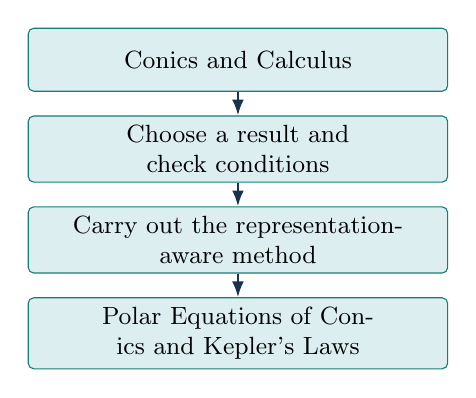
\begin{tikzpicture}[node distance=3mm, every node/.style={font=\small,align=center}, box/.style={draw=Teal,rounded corners=2pt,fill=Sky,minimum height=8mm,text width=0.42\textwidth}, arr/.style={-{Latex[length=2mm]},thick,draw=Ink}]
\node[box] (a) {Conics and Calculus};
\node[box,below=of a] (b) {Choose a result and check conditions};
\node[box,below=of b] (c) {Carry out the representation-aware method};
\node[box,below=of c] (d) {Polar Equations of Conics and Kepler's Laws};
\draw[arr] (a)--(b); \draw[arr] (b)--(c); \draw[arr] (c)--(d);
\end{tikzpicture}
\end{center}
\end{minipage}

\section{Learning objectives}
\begin{enumerate}
\item Explain the central objects and hypotheses in 10.1 and 10.6.
\item Translate among algebraic, graphical, numerical, and verbal representations.
\item Select an appropriate formula or theorem before beginning symbolic work.
\item Carry out multi-step calculations while preserving domain, sign, orientation, and units.
\item Diagnose common errors by testing assumptions and checking the result independently.
\item Synthesize the chapter's methods into a reusable problem-solving workflow.
\end{enumerate}

\section{10.1 Conics and Calculus}
\begin{longtable}{C N}\cornellcuehead
\cornellcuerow{What is the governing idea in 10.1?}{Parabolas, ellipses, and hyperbolas are characterized by geometric definitions and standard equations whose parameters control focus and directrix data.}
\cornellcuerow{Which result should be recalled?}{\formula{\frac{x^2}{a^2}+\frac{y^2}{b^2}=1,\qquad c^2=a^2-b^2}}
\cornellcuerow{How should a problem be organized?}{Complete squares, identify the conic and axes, extract vertices and foci, and use implicit differentiation for tangent information.}
\cornellcuerow{What should be checked before accepting an answer?}{Confirm the hypotheses and domain, preserve units and orientation when relevant, and substitute or differentiate back into the defining relation.}
\end{longtable}
\begin{warningbox}Using the ellipse relation $c^2=a^2-b^2$ for a hyperbola reverses the sign.\end{warningbox}
\begin{sectionsummarybox}Parabolas, ellipses, and hyperbolas are characterized by geometric definitions and standard equations whose parameters control focus and directrix data. The operational habit is to complete squares, identify the conic and axes, extract vertices and foci, and use implicit differentiation for tangent information.\end{sectionsummarybox}
\section{10.2 Plane Curves and Parametric Equations}
\begin{longtable}{C N}\cornellcuehead
\cornellcuerow{What is the governing idea in 10.2?}{A parameter generates paired coordinates and can encode direction, repeated points, and motion that a single rectangular function cannot.}
\cornellcuerow{Which result should be recalled?}{\formula{x=f(t),\qquad y=g(t)}}
\cornellcuerow{How should a problem be organized?}{Identify the parameter interval and orientation, eliminate the parameter only when useful, and retain restrictions lost during elimination.}
\cornellcuerow{What should be checked before accepting an answer?}{Confirm the hypotheses and domain, preserve units and orientation when relevant, and substitute or differentiate back into the defining relation.}
\end{longtable}
\begin{warningbox}The same rectangular curve can have different parametric orientation or coverage.\end{warningbox}
\begin{sectionsummarybox}A parameter generates paired coordinates and can encode direction, repeated points, and motion that a single rectangular function cannot. The operational habit is to identify the parameter interval and orientation, eliminate the parameter only when useful, and retain restrictions lost during elimination.\end{sectionsummarybox}
\section{10.3 Parametric Equations and Calculus}
\begin{longtable}{C N}\cornellcuehead
\cornellcuerow{What is the governing idea in 10.3?}{Parametric derivatives compare component rates, and parametric integrals accumulate with respect to the chosen parameter.}
\cornellcuerow{Which result should be recalled?}{\formula{\frac{dy}{dx}=\frac{dy/dt}{dx/dt},\qquad \frac{d^2y}{dx^2}=\frac{d}{dt}(dy/dx)\big/\frac{dx}{dt}}}
\cornellcuerow{How should a problem be organized?}{Differentiate components, locate where $dx/dt$ vanishes, preserve orientation in bounds, and use the parametric arc-length element.}
\cornellcuerow{What should be checked before accepting an answer?}{Confirm the hypotheses and domain, preserve units and orientation when relevant, and substitute or differentiate back into the defining relation.}
\end{longtable}
\begin{warningbox}The second derivative is not simply $(d^2y/dt^2)/(d^2x/dt^2)$.\end{warningbox}
\begin{sectionsummarybox}Parametric derivatives compare component rates, and parametric integrals accumulate with respect to the chosen parameter. The operational habit is to differentiate components, locate where $dx/dt$ vanishes, preserve orientation in bounds, and use the parametric arc-length element.\end{sectionsummarybox}
\section{10.4 Polar Coordinates and Polar Graphs}
\begin{longtable}{C N}\cornellcuehead
\cornellcuerow{What is the governing idea in 10.4?}{Polar coordinates represent a point by signed radial distance and angle, so representations are nonunique.}
\cornellcuerow{Which result should be recalled?}{\formula{x=r\cos\theta,\quad y=r\sin\theta,\quad r^2=x^2+y^2}}
\cornellcuerow{How should a problem be organized?}{Test symmetry carefully, find zeros and extrema of $r$, account for negative radius, and trace one complete parameter interval.}
\cornellcuerow{What should be checked before accepting an answer?}{Confirm the hypotheses and domain, preserve units and orientation when relevant, and substitute or differentiate back into the defining relation.}
\end{longtable}
\begin{warningbox}Assuming $r\ge0$ or tracing too short an interval can omit or misorient parts of the curve.\end{warningbox}
\begin{sectionsummarybox}Polar coordinates represent a point by signed radial distance and angle, so representations are nonunique. The operational habit is to test symmetry carefully, find zeros and extrema of $r$, account for negative radius, and trace one complete parameter interval.\end{sectionsummarybox}
\section{10.5 Area and Arc Length in Polar Coordinates}
\begin{longtable}{C N}\cornellcuehead
\cornellcuerow{What is the governing idea in 10.5?}{Polar area accumulates sectors, while polar arc length combines radial and angular change.}
\cornellcuerow{Which result should be recalled?}{\formula{A=\frac12\int_{\alpha}^{\beta}r^2\,d\theta,\qquad L=\int\sqrt{r^2+(dr/d\theta)^2}\,d\theta}}
\cornellcuerow{How should a problem be organized?}{Sketch and find intersection angles, choose outer-minus-inner radii for area between curves, and avoid duplicate tracing.}
\cornellcuerow{What should be checked before accepting an answer?}{Confirm the hypotheses and domain, preserve units and orientation when relevant, and substitute or differentiate back into the defining relation.}
\end{longtable}
\begin{warningbox}Solving intersections only by equating radii can miss common points represented by different angles or signs.\end{warningbox}
\begin{sectionsummarybox}Polar area accumulates sectors, while polar arc length combines radial and angular change. The operational habit is to sketch and find intersection angles, choose outer-minus-inner radii for area between curves, and avoid duplicate tracing.\end{sectionsummarybox}
\section{10.6 Polar Equations of Conics and Kepler's Laws}
\begin{longtable}{C N}\cornellcuehead
\cornellcuerow{What is the governing idea in 10.6?}{A focus-directrix conic has a polar equation controlled by eccentricity, linking orbital geometry to inverse-square motion.}
\cornellcuerow{Which result should be recalled?}{\formula{r=\frac{ed}{1\pm e\cos\theta}}}
\cornellcuerow{How should a problem be organized?}{Identify focus orientation from the denominator, classify by $e$, locate vertices, and interpret geometric parameters in context.}
\cornellcuerow{What should be checked before accepting an answer?}{Confirm the hypotheses and domain, preserve units and orientation when relevant, and substitute or differentiate back into the defining relation.}
\end{longtable}
\begin{warningbox}The sign and sine-versus-cosine choice encode directrix orientation; memorizing one form without geometry is fragile.\end{warningbox}
\begin{sectionsummarybox}A focus-directrix conic has a polar equation controlled by eccentricity, linking orbital geometry to inverse-square motion. The operational habit is to identify focus orientation from the denominator, classify by $e$, locate vertices, and interpret geometric parameters in context.\end{sectionsummarybox}

\section{Definitions and theorem register}
\small
\begin{longtable}{@{}>{\RaggedRight\arraybackslash}p{0.24\textwidth}>{\RaggedRight\arraybackslash}p{0.40\textwidth}>{\RaggedRight\arraybackslash}p{0.29\textwidth}@{}}
\toprule
\textbf{Topic} & \textbf{Meaning and conditions} & \textbf{Canonical form}\\
\midrule\endhead
10.1 Conics and Calculus & Parabolas, ellipses, and hyperbolas are characterized by geometric definitions and standard equations whose parameters control focus and. & \adjustbox{max width=\linewidth}{\(\displaystyle \frac{x^2}{a^2}+\frac{y^2}{b^2}=1,\qquad c^2=a^2-b^2\)} \\\addlinespace[2pt]
10.2 Plane Curves and Parametric Equations & A parameter generates paired coordinates and can encode direction, repeated points, and motion that a single rectangular function cannot. & \adjustbox{max width=\linewidth}{\(\displaystyle x=f(t),\qquad y=g(t)\)} \\\addlinespace[2pt]
10.3 Parametric Equations and Calculus & Parametric derivatives compare component rates, and parametric integrals accumulate with respect to the chosen parameter. & \adjustbox{max width=\linewidth}{\(\displaystyle \frac{dy}{dx}=\frac{dy/dt}{dx/dt},\qquad \frac{d^2y}{dx^2}=\frac{d}{dt}(dy/dx)\big/\frac{dx}{dt}\)} \\\addlinespace[2pt]
10.4 Polar Coordinates and Polar Graphs & Polar coordinates represent a point by signed radial distance and angle, so representations are nonunique. & \adjustbox{max width=\linewidth}{\(\displaystyle x=r\cos\theta,\quad y=r\sin\theta,\quad r^2=x^2+y^2\)} \\\addlinespace[2pt]
10.5 Area and Arc Length in Polar Coordinates & Polar area accumulates sectors, while polar arc length combines radial and angular change. & \adjustbox{max width=\linewidth}{\(\displaystyle A=\frac12\int_{\alpha}^{\beta}r^2\,d\theta,\qquad L=\int\sqrt{r^2+(dr/d\theta)^2}\,d\theta\)} \\\addlinespace[2pt]
10.6 Polar Equations of Conics and Kepler's Laws & A focus-directrix conic has a polar equation controlled by eccentricity, linking orbital geometry to inverse-square motion. & \adjustbox{max width=\linewidth}{\(\displaystyle r=\frac{ed}{1\pm e\cos\theta}\)} \\\addlinespace[2pt]
\bottomrule
\end{longtable}
\normalsize

\section{Formula and method sheet}
\small
\begin{longtable}{@{}>{\RaggedRight\arraybackslash}p{0.08\textwidth}>{\RaggedRight\arraybackslash}p{0.48\textwidth}>{\RaggedRight\arraybackslash}p{0.37\textwidth}@{}}
\toprule
\textbf{Sec.} & \textbf{Method sequence} & \textbf{Stop-and-check trigger}\\
\midrule\endhead
10.1 & Complete squares, identify the conic and axes, extract vertices and foci, and use implicit differentiation for tangent information. & Using the ellipse relation $c^2=a^2-b^2$ for a hyperbola reverses the sign. \\\addlinespace[2pt]
10.2 & Identify the parameter interval and orientation, eliminate the parameter only when useful, and retain restrictions lost during elimination. & The same rectangular curve can have different parametric orientation or coverage. \\\addlinespace[2pt]
10.3 & Differentiate components, locate where $dx/dt$ vanishes, preserve orientation in bounds, and use the parametric arc-length element. & The second derivative is not simply $(d^2y/dt^2)/(d^2x/dt^2)$. \\\addlinespace[2pt]
10.4 & Test symmetry carefully, find zeros and extrema of $r$, account for negative radius, and trace one complete parameter interval. & Assuming $r\ge0$ or tracing too short an interval can omit or misorient parts of the curve. \\\addlinespace[2pt]
10.5 & Sketch and find intersection angles, choose outer-minus-inner radii for area between curves, and avoid duplicate tracing. & Solving intersections only by equating radii can miss common points represented by different angles or signs. \\\addlinespace[2pt]
10.6 & Identify focus orientation from the denominator, classify by $e$, locate vertices, and interpret geometric parameters in context. & The sign and sine-versus-cosine choice encode directrix orientation; memorizing one form without geometry is fragile. \\\addlinespace[2pt]
\bottomrule
\end{longtable}
\normalsize

\section{Common errors and diagnostic checks}
\begin{warningbox}
\begin{itemize}
\item \textbf{10.1:} Using the ellipse relation $c^2=a^2-b^2$ for a hyperbola reverses the sign.
\item \textbf{10.2:} The same rectangular curve can have different parametric orientation or coverage.
\item \textbf{10.3:} The second derivative is not simply $(d^2y/dt^2)/(d^2x/dt^2)$.
\item \textbf{10.4:} Assuming $r\ge0$ or tracing too short an interval can omit or misorient parts of the curve.
\item \textbf{10.5:} Solving intersections only by equating radii can miss common points represented by different angles or signs.
\item \textbf{10.6:} The sign and sine-versus-cosine choice encode directrix orientation; memorizing one form without geometry is fragile.
\end{itemize}
\end{warningbox}
\begin{checkbox}
Before accepting any result: state the relevant domain; check theorem hypotheses; estimate sign and scale; preserve units and orientation; and verify by substitution, differentiation, a limiting case, or a second representation.
\end{checkbox}

\section{Chapter synthesis}
Use rectangular, parametric, and polar representations to analyze curves, motion, conics, area, and arc length with representation-aware calculus. The chapter begins with \textbf{Conics and Calculus} and culminates in \textbf{Polar Equations of Conics and Kepler's Laws}. Across the sequence, the most reliable workflow is to identify the mathematical object, choose a representation, state the governing result with its hypotheses, compute without dropping restrictions, and audit the answer against the original definition. Coordinate systems are analytical choices: preserve parameter intervals, orientation, nonuniqueness, and geometric meaning when translating derivatives and integrals between representations.

\section{Self-test questions}
\begin{enumerate}
\item Explain the central distinction or object in 10.1, using both words and notation.
\item State the main formula or result from 10.2 and identify every hypothesis or restriction needed for its use.
\item Describe the problem-solving procedure for 10.3. What is the strongest independent check?
\item Compare the roles of Conics and Calculus and Polar Equations of Conics and Kepler's Laws within this chapter.
\item Reconstruct the governing formula for 10.4 from its geometric or analytic meaning.
\item Choose one method in the chapter and explain how its output should be interpreted, including units or orientation when applicable.
\item Scenario: A student working on 10.1 produces a polished calculation but makes this error: Using the ellipse relation $c^2=a^2-b^2$ for a hyperbola reverses the sign. Diagnose the earliest invalid step and repair the workflow.
\item Scenario: A solution in 10.2 quotes the displayed formula without checking conditions. Which conditions must be checked, and what could fail if they are absent?
\item Construct a concept map linking a representation, a governing result, a computation, and a verification check from this chapter.
\item Design a two-part test for mastery: one conceptual prompt and one calculation. State what evidence would count as a complete answer.
\end{enumerate}

\Needspace{8\baselineskip}
\section{Answer key}
\small
\begin{enumerate}
\item A complete response identifies Parabolas, ellipses, and hyperbolas are characterized by geometric definitions and standard equations whose parameters control focus and directrix data. It should connect that meaning to \(\frac{x^2}{a^2}+\frac{y^2}{b^2}=1,\qquad c^2=a^2-b^2\) and state the relevant domain.
\item The organizing result is \(x=f(t),\qquad y=g(t)\). The solver must check that the quantities are defined and that the assumptions named in 10.2 hold before applying it.
\item Use this sequence: Differentiate components, locate where $dx/dt$ vanishes, preserve orientation in bounds, and use the parametric arc-length element. The strongest check is to return to the defining relation or differentiate/substitute the result, as appropriate.
\item Conics and Calculus establishes parabolas, ellipses, and hyperbolas are characterized by geometric definitions and standard equations whose parameters control focus and directrix data. Polar Equations of Conics and Kepler's Laws extends the chapter to a focus-directrix conic has a polar equation controlled by eccentricity, linking orbital geometry to inverse-square motion. The connection is the reuse of the same representations under a broader method.
\item The formula \(x=r\cos\theta,\quad y=r\sin\theta,\quad r^2=x^2+y^2\) follows by translating the defining geometric or rate relationship into symbols; each factor records a distinct change or scale.
\item Interpretation must name what varies, with respect to what, and on which domain. A numerical value without units, sign, direction, or interval information is incomplete whenever those features are part of the modeled quantity.
\item The earliest fault is the unverified assumption described by this warning: Using the ellipse relation $c^2=a^2-b^2$ for a hyperbola reverses the sign. Restart by following this procedure: Complete squares, identify the conic and axes, extract vertices and foci, and use implicit differentiation for tangent information.
\item The formula \(x=f(t),\qquad y=g(t)\) is conditional, not decorative. Check domain, differentiability or integrability as relevant, boundary or orientation requirements, and nonzero denominators before drawing a conclusion.
\item One valid map is: the representation in 10.1 identifies the object; the result in 10.2 supplies a rule; the method in 10.3 carries out the computation; the check in 10.6 tests the conclusion against its definition.
\item The conceptual prompt should require explanation of a definition and its hypotheses. The calculation should require method selection rather than direct substitution. Full evidence includes setup, justified transformations, a result, and an independent check.
\end{enumerate}
\normalsize

\section{Key-term recap}
\small
\begin{longtable}{@{}>{\RaggedRight\arraybackslash}p{0.29\textwidth}>{\RaggedRight\arraybackslash}p{0.64\textwidth}@{}}
\toprule
\textbf{Term} & \textbf{Working meaning}\\
\midrule\endhead
Conics and Calculus & Parabolas, ellipses, and hyperbolas are characterized by geometric definitions and standard equations whose parameters control focus and directrix data. \\\addlinespace[2pt]
Plane Curves and Parametric Equations & A parameter generates paired coordinates and can encode direction, repeated points, and motion that a single rectangular function cannot. \\\addlinespace[2pt]
Parametric Equations and Calculus & Parametric derivatives compare component rates, and parametric integrals accumulate with respect to the chosen parameter. \\\addlinespace[2pt]
Polar Coordinates and Polar Graphs & Polar coordinates represent a point by signed radial distance and angle, so representations are nonunique. \\\addlinespace[2pt]
Area and Arc Length in Polar Coordinates & Polar area accumulates sectors, while polar arc length combines radial and angular change. \\\addlinespace[2pt]
Polar Equations of Conics and Kepler's Laws & A focus-directrix conic has a polar equation controlled by eccentricity, linking orbital geometry to inverse-square motion. \\\addlinespace[2pt]
\bottomrule
\end{longtable}
\normalsize

\enlargethispage{4\baselineskip}
\begin{tcolorbox}[title=One-sentence takeaway,fonttitle=\bfseries,colback=Ink,colframe=Ink,coltext=white,coltitle=white,arc=2mm,boxrule=0pt]
\centering\bfseries Coordinate systems are analytical choices: preserve parameter intervals, orientation, nonuniqueness, and geometric meaning when translating derivatives and integrals between representations.
\end{tcolorbox}
\end{document}
